\documentclass[10pt,t,english]{beamer}
\usepackage{fontawesome}
\usepackage{graphicx}
\usepackage{array}
\usepackage[normalem]{ulem}
\usepackage{amsfonts,amsmath,amssymb,bm,bbm}
\usepackage{mathrsfs}
\usepackage{sgame}
\usepackage{graphicx,pstricks}
\usepackage{xcolor}
\usepackage{colortbl}
\usepackage{makecell}
\usepackage{tikz,tikzsymbols,gnuplottex}
\usetikzlibrary{decorations.pathreplacing,shapes}
\usepackage[english]{babel}
\usepackage[utf8]{inputenc}
\usepackage{appendixnumberbeamer}
\usepackage{datetime2}
\usepackage{booktabs}
\usepackage{setspace}
\usepackage{rotating}
\usepackage{natbib}
\usepackage{listings}

%\usepackage{matlab-prettifier} % For enhanced MATLAB highlighting
\lstset{
    language=matlab,
    % Other options for styling (optional)
    basicstyle=\ttfamily\footnotesize, % Font style
    keywordstyle=\color{blue}, % Keyword color
    commentstyle=\color{green!50!black}, % Comment color
    stringstyle=\color{red!70!black}, % String color
    numbers=left, % Line numbers on the left
    numberstyle=\tiny\color{gray}, % Style for line numbers
    frame=single, % Frame around the listing
    breaklines=true, % Allow line breaking
    captionpos=b, % Caption at the bottom
    tabsize=4 % Tab size
}

% ------------------------------------------------------------------------------
% Use the beautiful metropolis beamer template
% ------------------------------------------------------------------------------
\usepackage[T1]{fontenc}
\usepackage[utf8]{inputenc}
\usepackage{fontawesome}
\usepackage{FiraSans} 
\mode<presentation>
{
  \usetheme[progressbar=foot,background=light]{metropolis} 
  \usecolortheme{default} % or try albatross, beaver, crane, ...
  \usefonttheme{default}  % or try default, serif, structurebold, ...
  \setbeamertemplate{navigation symbols}{}
  \setbeamertemplate{caption}[numbered]
  %\setbeamertemplate{frame footer}{My custom footer}
} 

\newenvironment{stepenumerate}{\begin{enumerate}[<+->]}{\end{enumerate}}
\newenvironment{stepitemize}{\begin{itemize}[<+->]}{\end{itemize} }
\newenvironment{stepenumeratewithalert}{\begin{enumerate}[<+-| alert@+>]}{\end{enumerate}}
\newenvironment{stepitemizewithalert}{\begin{itemize}[<+-| alert@+>]}{\end{itemize} }

\newtheorem{question}{Question}
\newtheorem{claim}{Claim}
\newtheorem{proposition}{Proposition}
\newtheorem{remark}{Remark}
\newtheorem{conjecture}{Conjecture}

\definecolor{metrop}{RGB}{29, 44, 44}
\colorlet{GrayLight}{black!15}
\colorlet{GrayMedium}{black!30}
\colorlet{ForestGreen}{green!60!black}

\newenvironment{transitionframe}{
  \setbeamercolor{background canvas}{bg=black!80}
  \begin{frame}}{
    \end{frame}
}

\newcommand{\br}{

\bigskip

}

\newcommand{\pd}{\partial}
\newcommand{\RR}{\mathbb{R}}

\newcommand*\hugme[1]{\tikz[baseline=(char.base)]{\node[shape=ellipse,draw,inner sep=0pt] (char) {#1};}}

\newcounter{saveenumi}
\newcommand{\seti}{\setcounter{saveenumi}{\value{enumi}}}
\newcommand{\conti}{\setcounter{enumi}{\value{saveenumi}}}
\resetcounteronoverlays{saveenumi}



\newcommand\dotprod[2]{\langle #1 , #2 \rangle}
\newcommand{\ft}[1]{\widehat #1}
\newcommand{\qabove}[1]{\overset{\text{\large \textbf ?}}{#1}}
\newcommand{\eqae}{\overset{\text{a.e.}}{=}}
\newcommand{\calp}{\mathcal{P}}
\newcommand{\calg}{\mathcal{G}}
\newcommand{\calb}{\mathcal{B}}
\newcommand{\textd}{\text{d}}
\newcommand{\bbr}{\mathbb{R}}
\newcommand{\binm}{\mathbin{M}}
\newcommand{\binc}{\mathbin{C}}
\newcommand{\binb}{\mathbin{B}}
\newcommand{\calc}{\mathcal{C}}
\newcommand{\calh}{\mathcal{H}}
\newcommand{\bfone}{\mathbf{1}}
\newcommand{\bbe}{\mathbb{E}}
\newcommand{\bfle}{\mathbf{e}}
\newcommand{\calf}{\mathcal{F}}
\newcommand{\cala}{\mathcal{A}}
\newcommand{\cale}{\mathcal{E}}
\newcommand{\bbn}{\mathbb{N}}
\newcommand{\cantor}{\calc}
\newcommand{\calY}{\mathcal{Y}}
\newcommand{\textb}{\text{B}}
\newcommand{\calm}{\mathcal{M}}
\newcommand{\bint}{\mathbin{T}}
\newcommand{\ep}{\epsilon}
\newcommand{\bbq}{\mathbb{Q}}
\newcommand{\bbp}{\mathbb{P}}
\newcommand{\cals}{\mathcal{S}}
\newcommand{\emptysequence}{e}
\newcommand{\bbz}{\mathbb{Z}}
\newcommand{\fraka}{\frak{A}}
\newcommand{\frakb}{\frak{B}}
\newcommand{\length}{\text{length}}
\newcommand{\bfn}{\mathbf{N}}
\newcommand{\support}{\text{support}}
\DeclareMathOperator*{\argmax}{arg\,max}
\newcommand{\dom}{\mbox{dom}}
\def\ut{\underline t}
\def\um{\underline m}
\def\PP{\mathbb{P}}
\def\EE{\mathbb{E}}
\def\RR{\mathbb{R}}

% Title page info
\title[Incentives in Experiments: Theory]{ExpEcon Methods:\\Empirical Tests of Incentive Compatibility}
\author[ECON 8877]{ECON 8877\\P.J. Healy} \color{metrop}
\institute[OSU]{}
\date[]{\vfill {\tiny Updated \today\ at\ \DTMcurrenttime}}

\begin{document}

\frame{\maketitle}


\begin{frame}
  \frametitle{Testing IC vs. Framing Effects}
    A test of IC? (Cox Sadiraj \& Schmidt 2014)\\
    \begin{tabular}{|r||c|c|}
    \hline
                & $D_1$ & $D_2$ \\
    \hline
    Treatment 1: &    $\{\$4,(\frac{1}{2},\$10)\}$ & \\
    \hline
    Treatment 2: & $\{\$4,(\frac{1}{2},\$10)\}$ & $\{\$3,(\frac{1}{2},\$12)\}$ \\
    \hline
    \end{tabular}\\
    If we observe differences on $D_1$, it could be
    \begin{itemize}
      \item the mechanism was not IC, or
      \item the presence of $D_2$ altered preferences (e.g., decoy effect).
    \end{itemize}
    \br
    Other papers that use this method:
    \begin{itemize}
      \item Cubitt Starmer Sugden (1998 Exp.1)
      \item Beattie \& Loomes (1997)
      \item Cubitt Starmer Sugden (1998 Exp.2)
      \item Harrison \& Swarthout (2014)
      \item Cox Sadiraj \& Schmidt (2015)
    \end{itemize}
\end{frame}

\begin{frame}
  \frametitle{Tests Without Framing Confound}
    Replace Treatment 1 with a ``Framed Control'' treatment:\br
    \begin{tabular}{|r||c|c||l|}
    \hline
                & $D_1$ & $D_2$ & Mechanism \\
    \hline
    Treatment 1: & $\{\$4,(\frac{1}{2},\$10)\}$ & $\{\$3,(\frac{1}{2},\$12)\}$ & Pay only $D_1$ \\
    \hline
    Treatment 2: & $\{\$4,(\frac{1}{2},\$10)\}$ & $\{\$3,(\frac{1}{2},\$12)\}$ & RPS \\
    \hline
    \end{tabular}\br
  \textbf{\textcolor{red}{LESSON: Proper test of IC must show all subjects same choices.}}\br
  \vspace{1in}
\end{frame}


\begin{frame}{Cox, Sadiraj \& Schmidt (2015)}
Test various payment mechanisms in lottery choice setting
\begin{enumerate}
    \item Pay All (PA)
    \begin{itemize}
        \item PAS: Sequentially (learn outcome each period)
        \item PAI: Independently at the end
    \end{itemize}
    \item Pay One Randomly (POR)
    \begin{enumerate}
        \item PORpi: with prior info about all choices to be made
        \item PORnp: no info about upcoming choices
        \item PORpas: learn realized payoffs you go, then get 1 at the end
    \end{enumerate}
    \item Pay All Correlated (PAC) (lotteries must have same state space)
    \begin{itemize}
        \item PAC/N divides payoffs by \# of decisions, to match POR
    \end{itemize}
    \item One Task (OT)
    \begin{enumerate}
        \item ImpureOT: Make all choices, but only one is paid
        \begin{itemize}
            \item Added by a referee (not me!) and reported separately
        \end{itemize}
    \end{enumerate}
\end{enumerate}
\end{frame}

\begin{frame}{Cox, Sadiraj \& Schmidt (2015)}
Design:
\begin{itemize}
    \item Choice over 5 lottery pairs
    \item Testing various versions of Allais paradox
    \item OT: between-subjects. All others: within-subject
    \begin{itemize}
        \item Therefore OT Allais paradoxes are between-subject via Probit
    \end{itemize}
    \item Choices on 5 separate slips of paper in an envelope
\end{itemize}
Analyses:
\begin{itemize}
    \item Probit on Pr(Allais paradox) including demographics, EV, etc.
    \item Choice frequencies
    \item Probit on choice frequencies
\end{itemize}
\end{frame}

\begin{frame}{Cox, Sadiraj \& Schmidt (2015)}
    \begin{center}
        \includegraphics[width=4in]{LectureSlides/graphics/mono/CoxEtAl1.png}
    \end{center}
    Can't really compare cleanly to OT\\
    But, definite differences across mechanisms\\
    And whether they see the questions in advance or not!
\end{frame}


\begin{frame}{Cox, Sadiraj \& Schmidt (2015)}
    \begin{center}
        \includegraphics[width=4in]{LectureSlides/graphics/mono/CoxEtAl2.png}
    \end{center}
    All Pairs: \% who chose safe in all 5
    Most risk averse: PORnp and PAI\\
    Least risk averse: PORpas and PAS
\end{frame}

\begin{frame}{Cox, Sadiraj \& Schmidt (2015)}
What about Impure OT?
\begin{itemize}
    \item Paper only compares Impure OT to OT
    \begin{itemize}
        \item More risky choices under Impure OT
        \item Framing effect exists!
    \end{itemize}
    \item But we want Impure OT vs. each mechanism!
    \item Probit Pr(Safe) results:
    \begin{itemize}
        \item PORnp, PORpi, and PAI are different from ImpureOT
    \end{itemize}
    \item But, looking at the actual choice data task-by-task, I don't find significant differences...
\end{itemize}
\end{frame}

\begin{frame}{Starmer \& Sugden (1991)}
\begin{itemize}
    \item 22 binary lottery choice questions. $n=40$ per treatment
    \item First 20: hypothetical (piloting for another study)
    \item Questions 21 and 22: RPS vs. only one paid. Same page.
    \item Allais paradox questions.
\end{itemize}    
\begin{center}
    \includegraphics[width=3.5in]{LectureSlides/graphics/mono/StarmerSugden1.png}
\end{center}
A vs. B: $p=0.356$ (my calculation)\\
C vs. D: $p=0.043$ (my calculation)
\end{frame}

\begin{frame}{Cubitt Starmer \& Sugden (1998)}
    \begin{itemize}
        \item Five binary menus of lotteries
        \item Experiment 1 ($n=201$)
        \begin{itemize}
            \item Group 1.1: RPS: $(1/3,D_3;2/3,D_4)$
            \item Group 1.2: RPS: $(1/3,D_3;2/3,D_5)$
            \item (Two other groups to test IND and ROCL)
            \item Use $D_3$ to test IC. No differences. 
        \end{itemize}
        \item Experiment 3 ($n=202$)
        \begin{itemize}
            \item 3.1: 20 decisions, 1st is paid
            \item 3.2: 20 decisions, 2nd is paid
            \item 3.3: 20 decisions, RPS on all 20
            \item 3.4: Same as 3.3 but with lower stakes
            \item 3.1 $D_1$ vs 3.3 $D_1$: $p=0.685$
            \item 3.2 $D_2$ vs 3.3 $D_2$: $p=0.120$
        \end{itemize}
    \end{itemize}
\end{frame}


\begin{frame}
  \frametitle{Summary of Past Experiments}
  \begin{center}
        \includegraphics[width=3.5in]{LectureSlides/graphics/mono/BrownHealyLitReview2.png}
  \end{center}
\end{frame}



\begin{frame}
  \frametitle{Brown \& Healy (2018)}
  \centering
  \begin{figure}
    \includegraphics[width=3.5in]{LectureSlides/graphics/mono/ScreenShotL2.png}
  \end{figure}
\end{frame}


\begin{frame}
  \frametitle{Our Design}
  \centering
  \begin{figure}
    \includegraphics[width=4.5in]{LectureSlides/graphics/mono/TreatmentList.png}
  \end{figure}
  \br
  \begin{itemize}
    \item Andreoni-Sprenger formatting
    \item Standard Ohio State subject pool.
    \item Between-subjects.
    \item Computerized.
    \begin{itemize}
        \item List format: rows must be answered sequentially.
    \end{itemize}
    \item Physical randomizing devices (die, bingo cage)
    \item No other tasks in the experiment.
    \item 60--63 subjects per treatment.
    \item Question: Do Row 14 choices differ by treatment?
  \end{itemize}
\end{frame}

\begin{frame}
  \frametitle{The Results}
  Row 14:\\
    \centering
  \begin{figure}
    \includegraphics[width=4.5in]{LectureSlides/graphics/mono/ResultsList.png}
  \end{figure}
  \br
  \begin{itemize}
    \item Using RPS mechanism makes them switch later.\\(More thoughtful? Switching inertia?)
    \begin{itemize}
      \item Statistically significant.
    \end{itemize}
    \item Showing whole list makes them switcher earlier\\(Closer to the middle.)
    \begin{itemize}
      \item Not quite significant.
    \end{itemize}
    \item The two effects nearly offset

  \end{itemize}
\end{frame}

\begin{frame}
  \frametitle{Hypothesis}
    \begin{itemize}
      \item Subjects are combining the decisions in a reduction-like way.\\\emph{E.g.}: `When to switch?'.
      \item The `combining' can be broken by separating the decisions.
    \end{itemize}
\end{frame}

\begin{frame}
  \frametitle{New Treatments}
  `Separated' treatments.
  \begin{itemize}
    \item Same 20 rows.
    \item Each shown on separate screen.
    \item Order of rows randomized for each subject.
    \item Still comparing RPS to Pay-14-Only.
    \item Still must answer every row, in order given.
    \begin{itemize}
        \item First attempt: on paper. They shirked.
        \item Second attempt: computerized, forced answers
    \end{itemize}
    \item Still 60--63 observations per cell, between subjects.
  \end{itemize}
\end{frame}

\begin{frame}
  \frametitle{Full Design}
  \centering
  \begin{figure}
    \includegraphics[width=4.5in]{LectureSlides/graphics/mono/TreatmentsAll.png}
  \end{figure}
\end{frame}


\begin{frame}
  \frametitle{The Results}
    \centering
  \begin{figure}
    \includegraphics[width=4.5in]{LectureSlides/graphics/mono/ResultsAll.png}
  \end{figure}
\end{frame}

\begin{frame}
  \frametitle{The Cost of Separation}
   B-to-A (Risky-to-Safe) switches violate FOSD:\\
   $Risky_{15}$ dominates $Risky_{14}$, but $Risky_{14} \succ Safe \succ Risky_{15}$\br
  \centering
  \includegraphics[width=3in]{LectureSlides/graphics/mono/BrownHealySwitchBacks.png}\\
  \textbf{\textcolor{red}{LESSON: Separating decisions hurts consistency? NO!\\The list format generates \emph{false consistency}!}}
\end{frame}

\begin{frame}{Biases Cancel Out}
\begin{center}
    \includegraphics[width=3in]{LectureSlides/graphics/mono/BrownHealyChoicesByRow.png}
\end{center}
L-RPS was fine because ``list effect'' and ``IC failure'' canceled out!\\
I wouldn't expect that to be true generally...
    
\end{frame}


\begin{frame}
  \frametitle{Past Experiments}
  \begin{center}
   \includegraphics[width=4.5in]{LectureSlides/graphics/mono/BrownHealyLitReview1.png}
  \end{center}
\end{frame}

\begin{frame}{Other Discussion of Separation}
\begin{enumerate}
    \item Kirby \& Marakovic (1996) and Kirby et al. (1999)
    \begin{itemize}
        \item Use scrambled lists in a field setting, including heroin addicts
    \end{itemize}
    \item Eckel et al. (2005)
    \begin{itemize}
        \item Use scrambled with working poor
        \item ``we now believe that scrambling is a bad idea because it results in greater inconsistency and variance of responses.''
    \end{itemize}
\end{enumerate}
\end{frame}

\begin{frame}{RPS for Hedging Ambiguity?}
Is RPS used to hedge ambiguity?
    \begin{itemize}
        \item Oechssler Rau \& Roomets (2019): No
        \begin{itemize}
            \item Issues with their design
        \end{itemize}
        \item Baillon Halevy \& Li (2022)...
    \end{itemize}
\end{frame}

\begin{frame}[t]{2-Urn Ellsberg Paradox}
\begin{center}
    \includegraphics[width=2in]{LectureSlides/graphics/mono/twojars.png}\\
\begin{tabular}{|r|l|}
\hline
\multirow{2}{*}{\color{red}$D_1$:} & {\color{red}K} $=$ \$2.00 if {\color{red} red} from K \\
%\cline{2}
 & {\color{red}U} $=$ \$2.10 if {\color{red}red} from U \\
 \hline
\multirow{2}{*}{\color{blue}$D_2$:} & {\color{blue}K} $=$ \$2.00 if {\color{blue}blue} from K \\
%\cline{2}
 & {\color{blue}U} $=$ \$2.10 if {\color{blue}blue} from U \\
\hline
\multicolumn{2}{c}{One paid randomly via coin flip}
\end{tabular}
\end{center}

\textbf{Pr(Red in U)$\approx$Pr(Blue in U) \& Ambiguity Averse:} {\color{red}K} $\succ$ {\color{red}U} and {\color{blue}K} $\succ$ {\color{blue}U}.
\br
\textbf{Raiffa (1961):} Picking {\color{red}U}{\color{blue}U} ``hedges away'' the ambiguity! {\color{red}U}{\color{blue}U} $\succ$ {\color{red}K}{\color{blue}K}
\end{frame}

{
\setbeamercolor{background canvas}{bg=white}
\begin{frame}{How Hedging Works (Raiffa 1961)}
Picking {\color{red}U}{\color{blue}U}:
    \begin{center}
        \begin{tabular}{ccc}
            Original: & & Order-Reversed: \\
            \includegraphics[width=2in]{LectureSlides/graphics/mono/trees_coinfirst_2.png} &              & \includegraphics[width=2in]{LectureSlides/graphics/mono/trees_ballfirst.png}\\
             & & \\
             Ambiguity: & & 50-50 Lottery For Sure \\
             {\color{red}K}{\color{blue}K} $\succ$ {\color{red}U}{\color{blue}U} & & {\color{red}U}{\color{blue}U} $\succ$ {\color{red}K}{\color{blue}K} \\
                            & & \onslide<2>{\textbf{Assumption:} Order Reversal}
        \end{tabular}
    \end{center}
\end{frame}
}

\begin{frame}{Past Experiments}
Order reversal has support...
\begin{itemize}
    \item Coin before $\sim$ Coin after
    \begin{itemize}
        \item Oechssler, Rau \& Roomets (2019; ORR19)
        \item Baillon, Halevy \& Li (2022)
        % \item ``Order Reversal'' ($\Rightarrow$ complete separability??)
        %\item We should expect hedging (picking {\color{red}U}{\color{blue}U})
    \end{itemize}
\end{itemize}

\br

...yet people don't seem to appreciate hedging:
\begin{itemize}
    \item Raiffa (1961), Dominiak \& Schnedler (2011)
    \begin{itemize}
        \item Ambiguity averse subjects don't value {\color{red}U}{\color{blue}U} more than {\color{red}U} and {\color{blue}U}
    \end{itemize}
    \item ORR19 find mixed evidence for hedging
    \begin{itemize}
        \item Amb. Averse \& Pr(blue)$\approx$Pr(red) Subjects: 
        \begin{itemize}
            \item 50\% consistent with hedging (or randomization)
            \item Issues: Indifference \& Cross-task contamination
        \end{itemize}
    \end{itemize}
\end{itemize}
\end{frame}


\begin{frame}[t]{Past Experiments}
Baillon, Halevy \& Li (2022) (BHL22):
\begin{itemize}
    \item ``Single'' Treatment:
    \begin{itemize}
        \item $D_0=\{${\color{red}K},{\color{blue}K},{\color{red}U},{\color{blue}U}$\}$
        \item {\color{red}U} or {\color{blue}U} $\Rightarrow$ Ambiguity neutral/loving \textit{or} Pr(red)$\gtrless$Pr(blue)  \item {\color{red}K} or {\color{blue}K} $\Rightarrow$ Strictly ambiguity averse \textit{and} Pr(red)$\approx$Pr(blue) 

        \item 50\% choose {\color{red}K} or {\color{blue}K}\\
        $\Rightarrow$ 50\% are Amb. Averse \textit{and} Pr(red)$\approx$Pr(blue)\\
        \phantom{$\Rightarrow$} this is a \textit{lower bound} on Amb. Aversion
    \end{itemize}
    \item ``Before'' Treatment:
    \begin{itemize}
        \item $D_1=\{${\color{red}K},{\color{red}U}$\}$, $D_2=\{${\color{blue}K},{\color{blue}U}$\}$, coin flip \textbf{first}
        \item What will Amb. Averse subjects pick?
        \begin{itemize}
            \item Order Reversal + Hedging $\Rightarrow$ {\color{red}U}{\color{blue}U}
            \item ``Isolation'' $\Rightarrow$ {\color{red}K}{\color{blue}K}
            \item Pr(red)$\gtrless$Pr(blue) $\Rightarrow$ {\color{red}U}{\color{blue}K} or {\color{red}K}{\color{blue}U}\\
            (uses Azrieli et al. 2018, ignoring stochastic choice)
        \end{itemize}
    \end{itemize}
\end{itemize}

    
\end{frame}

\begin{frame}{BHL22: Results}
    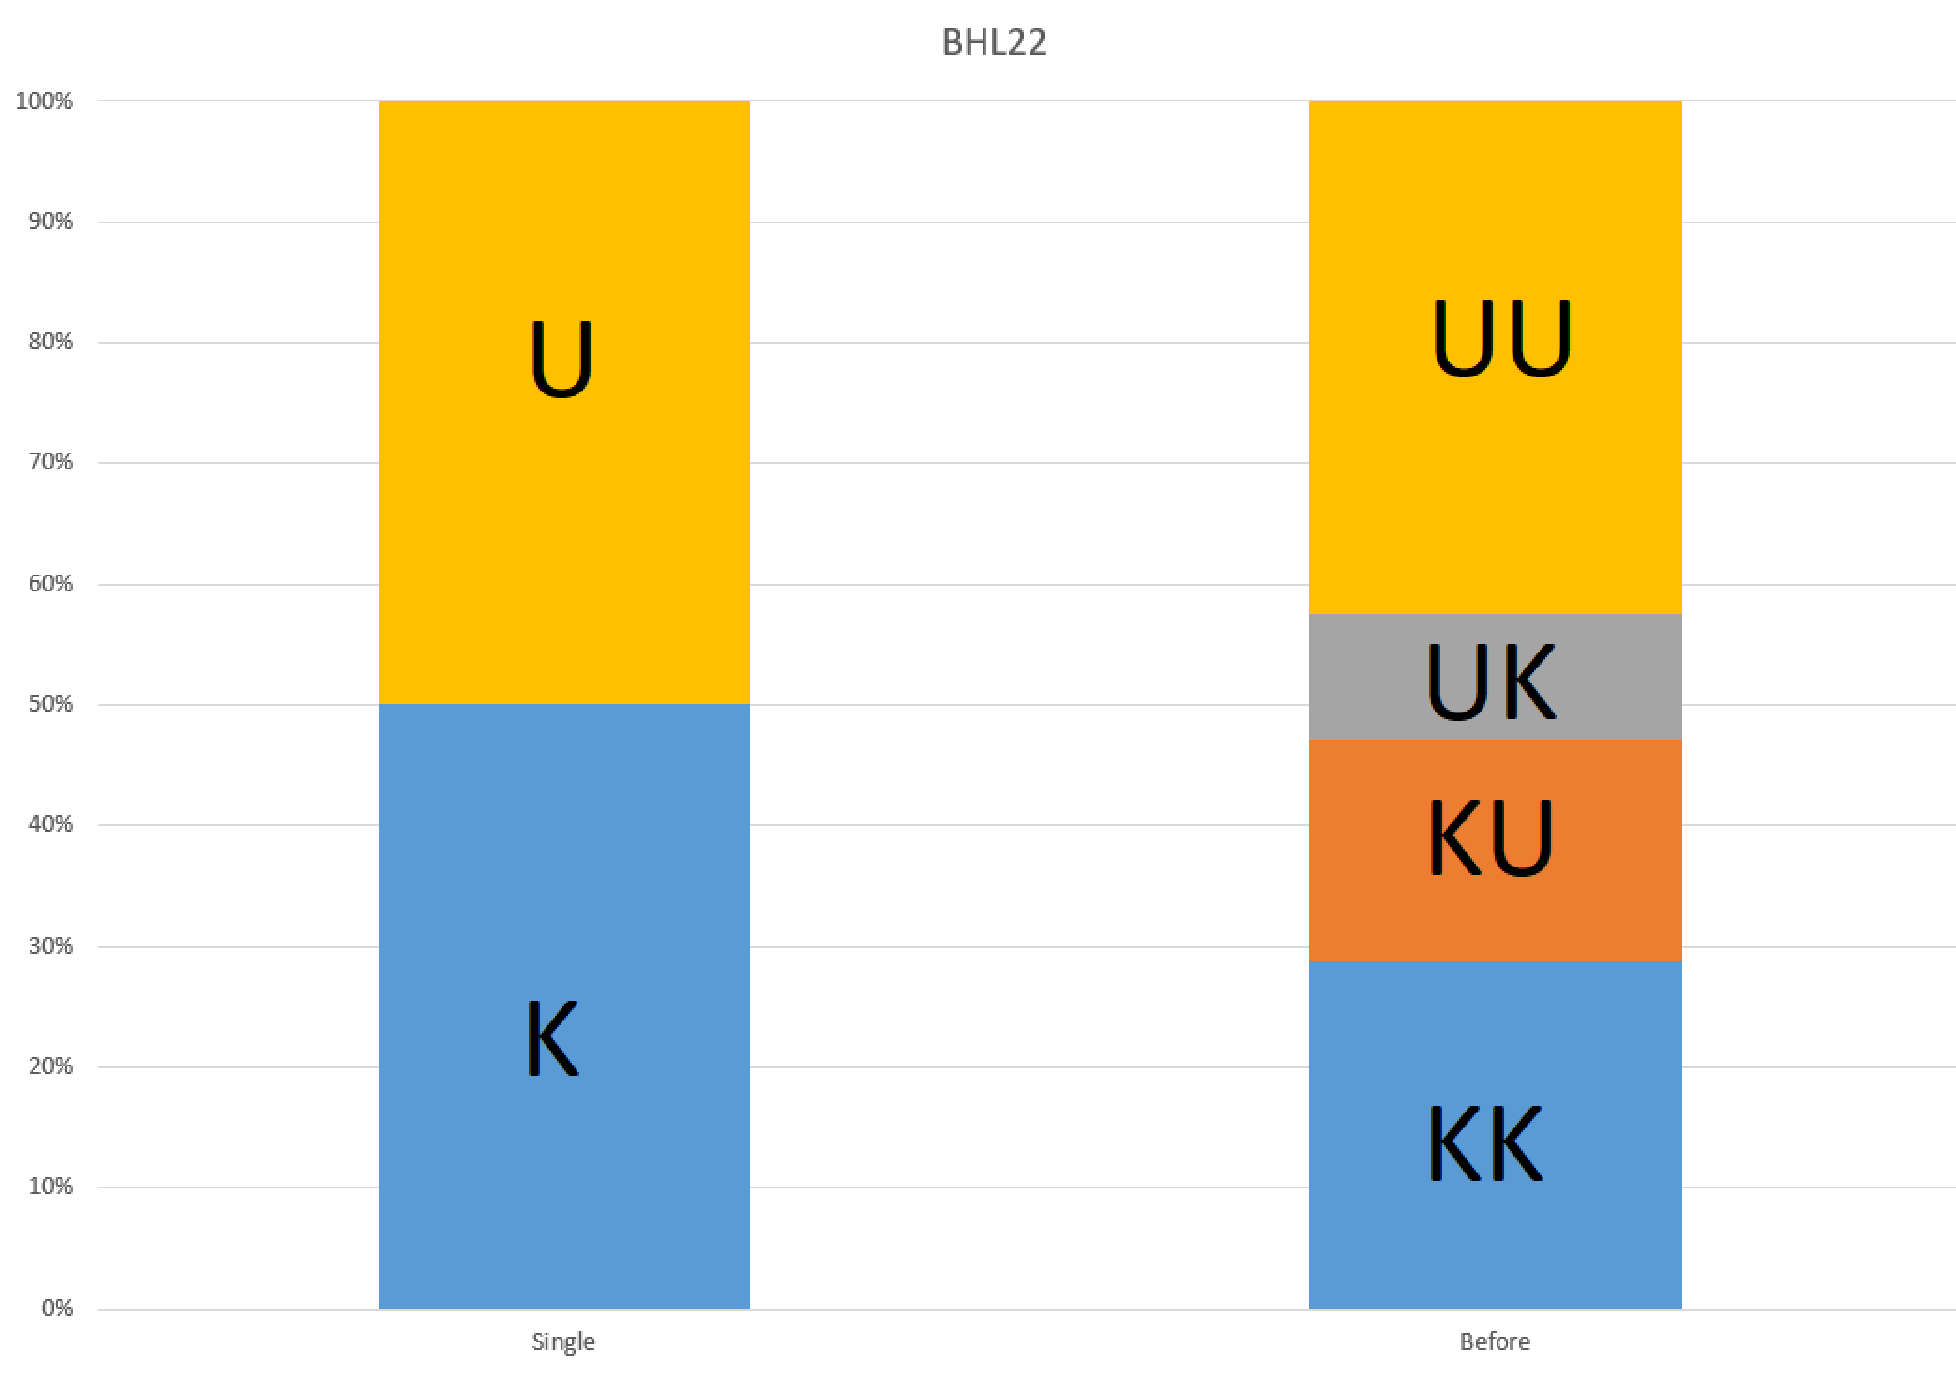
\includegraphics[width=4in]{LectureSlides/graphics/mono/BHL22_Stacked_Raw.pdf}
\end{frame}

\begin{frame}{BHL22: Story 1}
    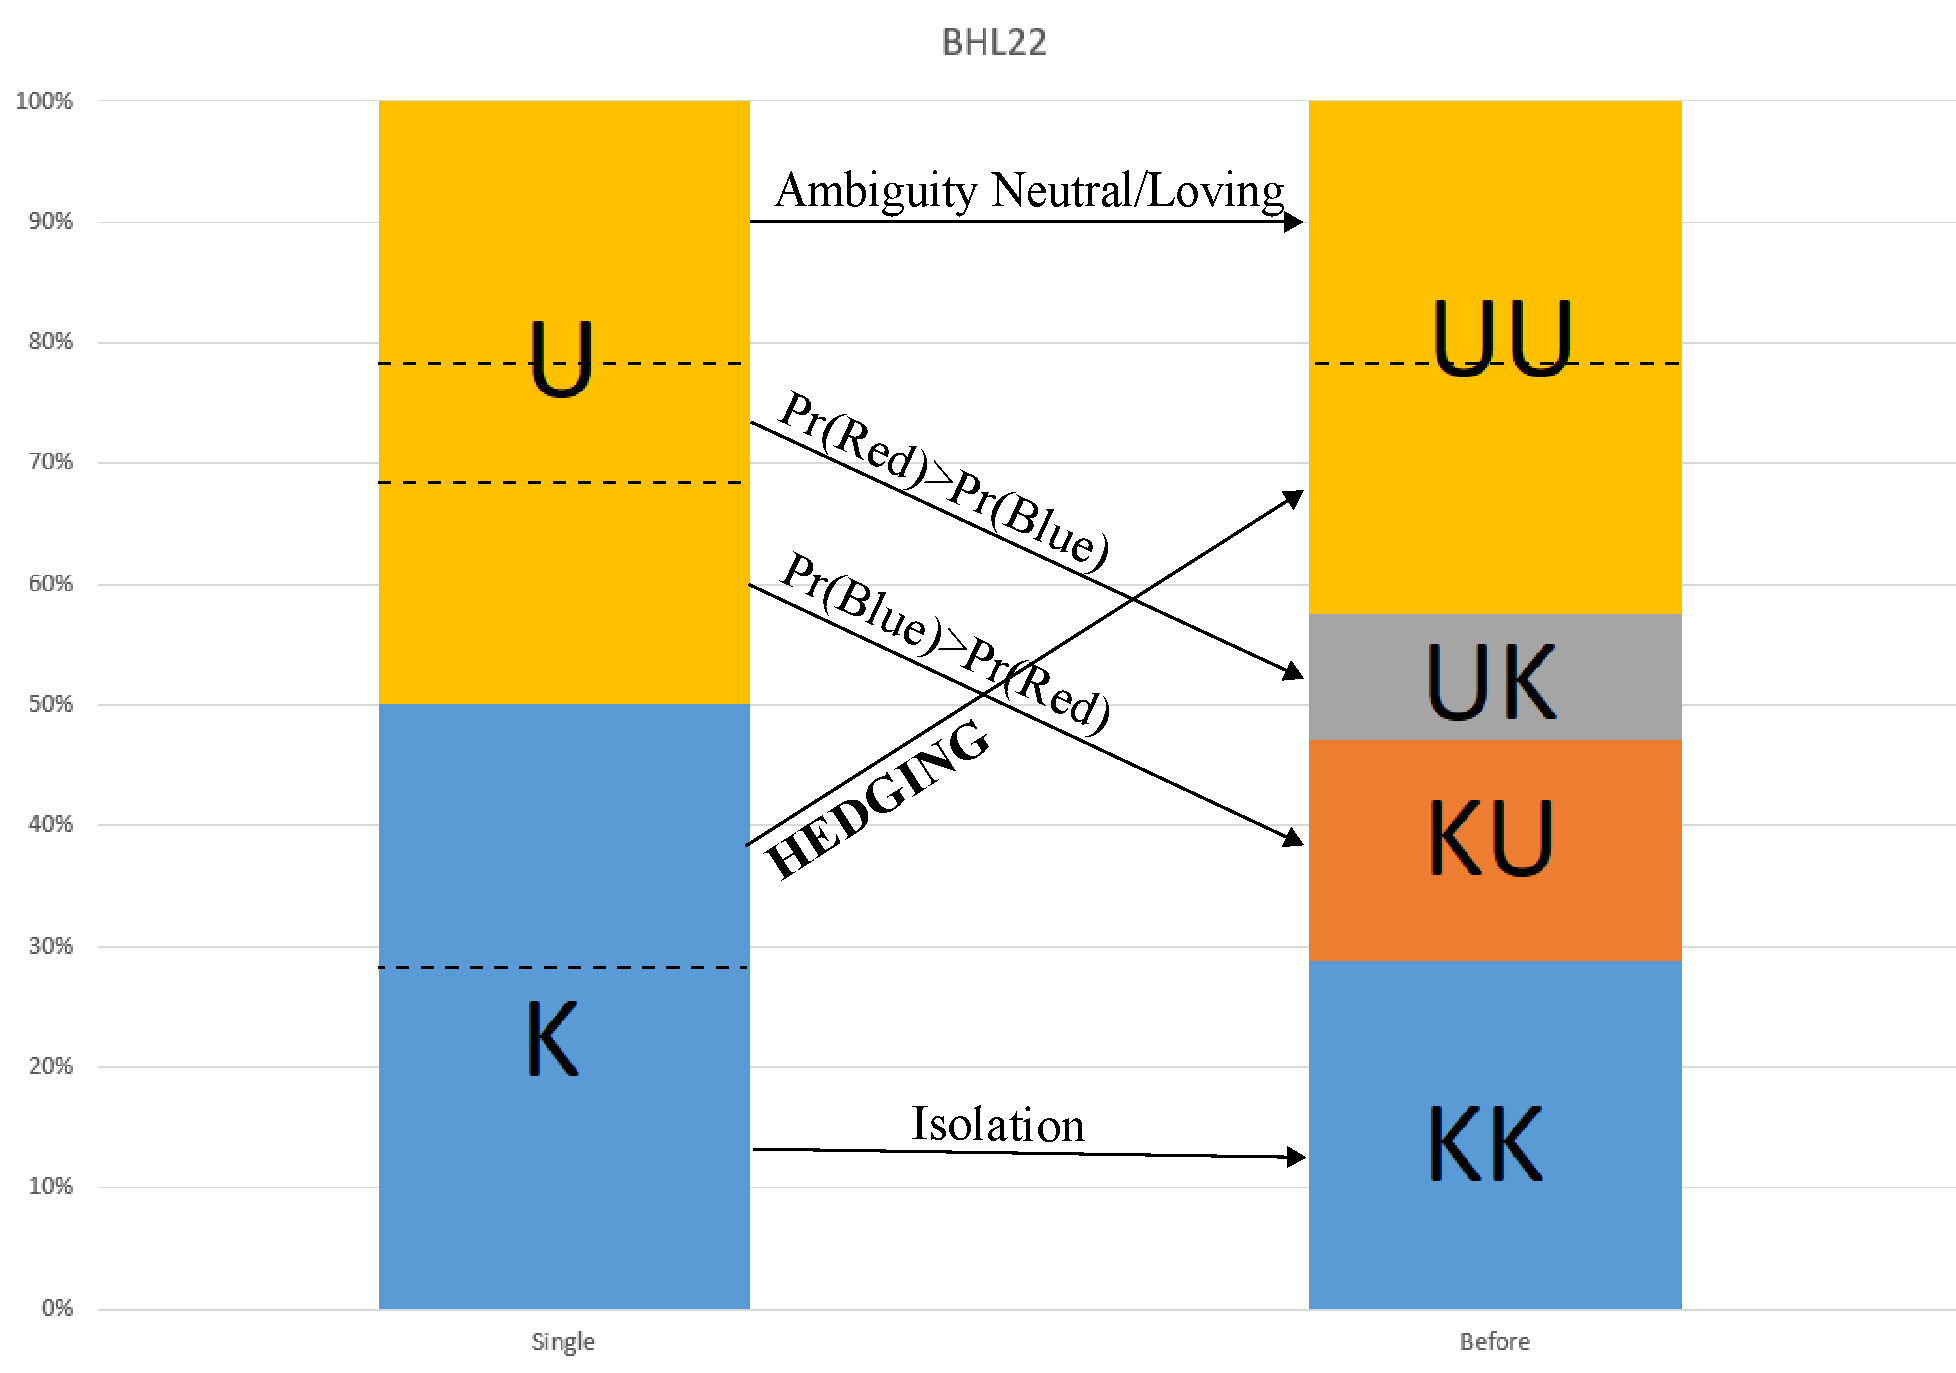
\includegraphics[width=4in]{LectureSlides/graphics/mono/BHL22_Stacked.pdf}
\end{frame}

\begin{frame}{BHL22: Story 2}
    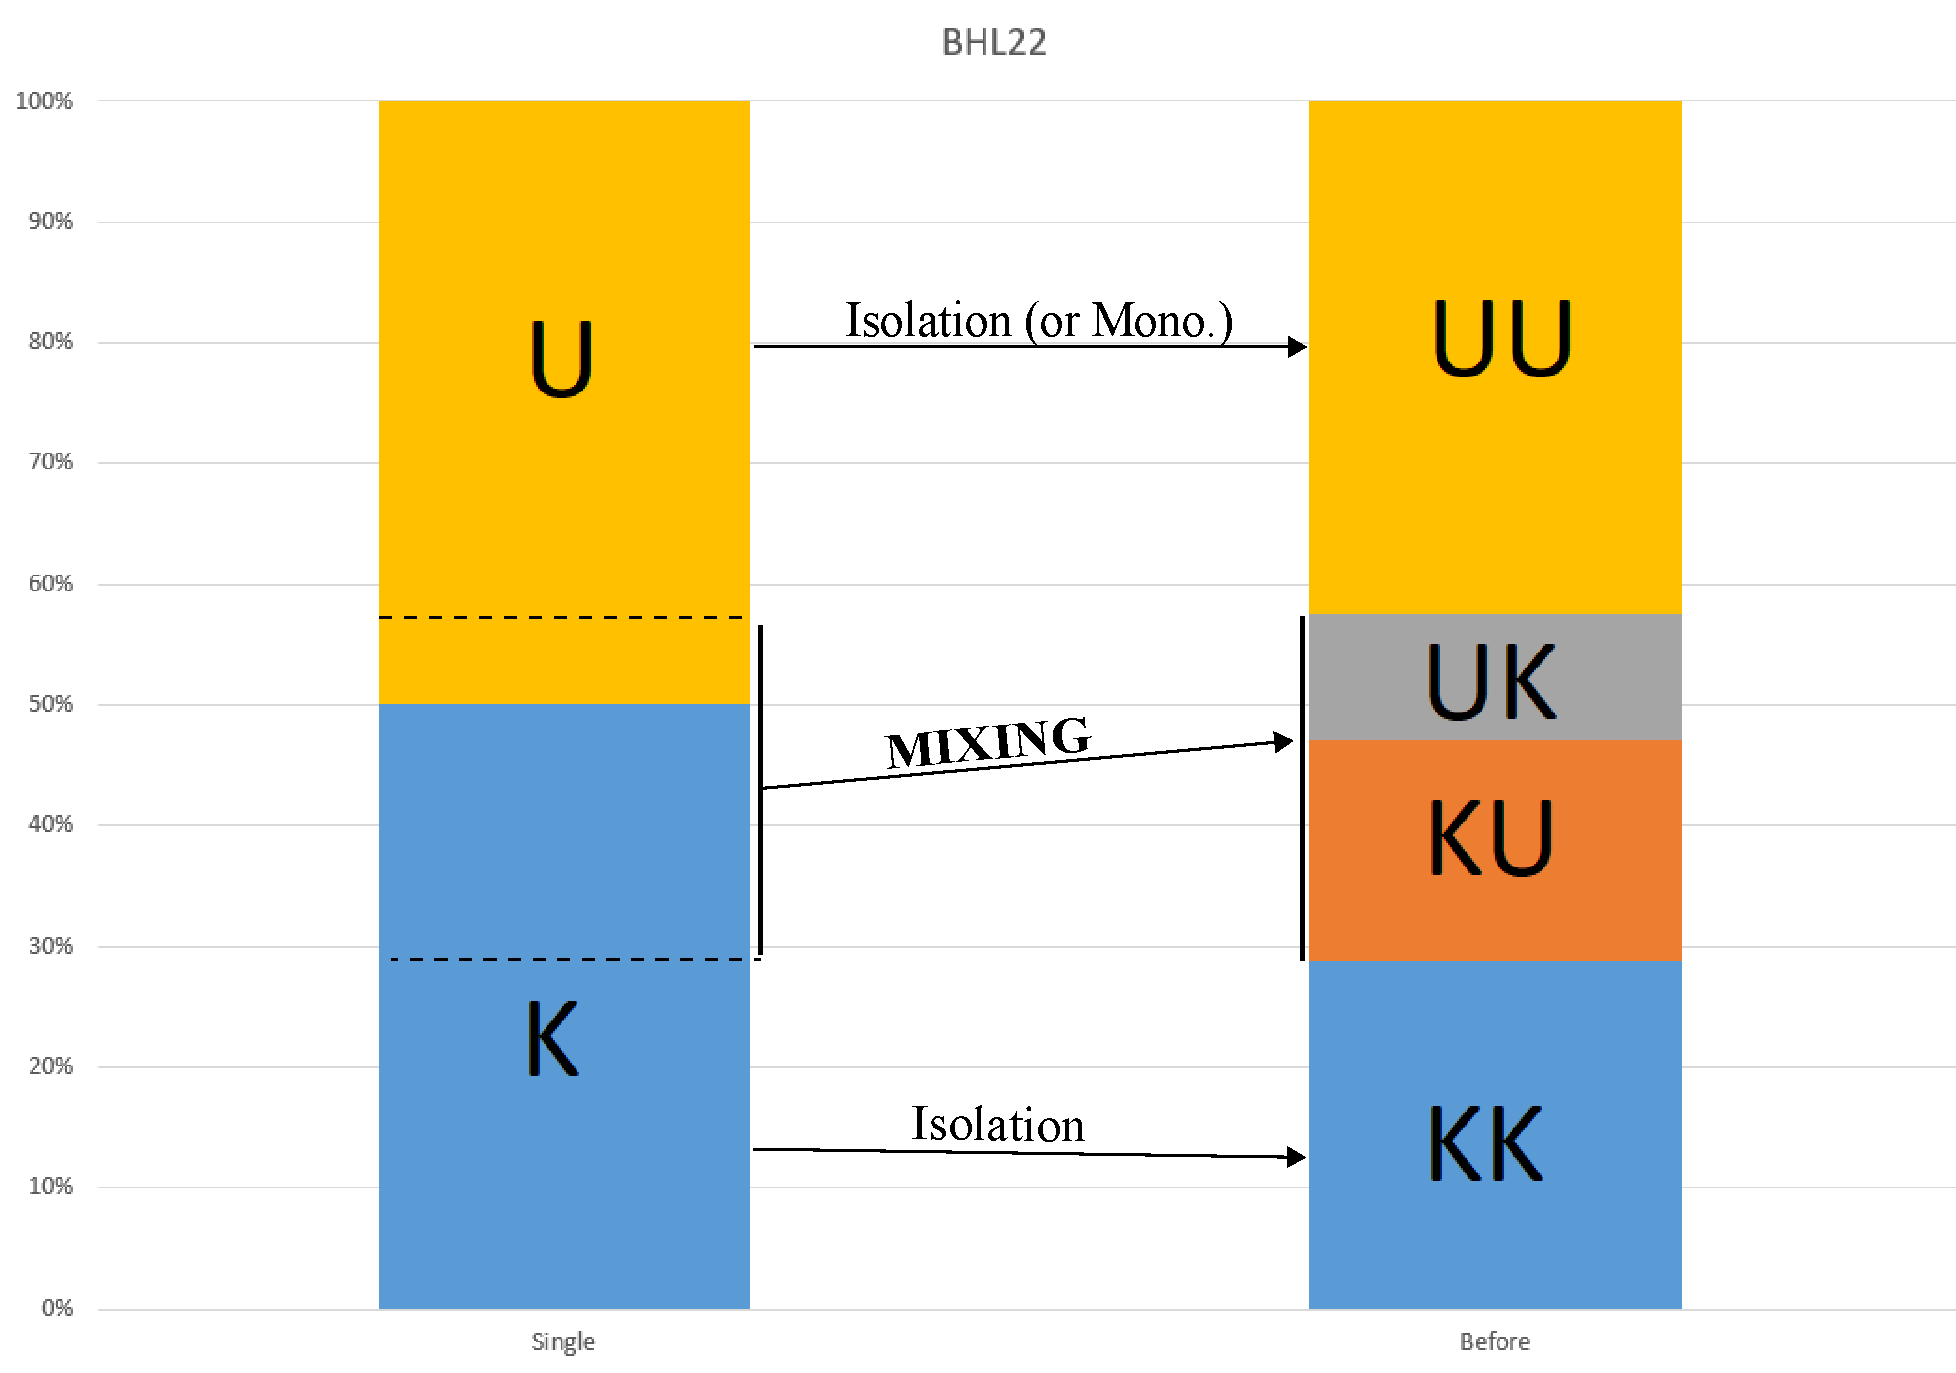
\includegraphics[width=4in]{LectureSlides/graphics/mono/BHL22_Stacked_Mixing.pdf}
Is it necessarily hedging?
\end{frame}

\begin{frame}{Pay All}
    Susan Laury's paper...    
\end{frame}

\begin{frame}
  \frametitle{Summary}
  \begin{itemize}
    \item Theory: RPS generally fine \emph{unless} subjects ``reduce''\\
          (treat the experiment as one large decision)
    \item List format seems to encourage reduction, IC violations
    \item Separated format breaks reduction, restores IC
    \begin{itemize}
      \item Separated \emph{and} random order. Haven't tested which.
    \end{itemize}
    \item List format generates \emph{false consistency}
    \item Ambiguity:
    \begin{itemize}
        \item RPS is not IC!
        \item But is it really hedging??
    \end{itemize}
  \end{itemize}
\end{frame}



\end{document}